% Megatron-Core MLP block (fc1 -> activation -> fc2) on one of p TP ranks, sequence parallel ON.
% Grounded in NVIDIA/Megatron-LM @ e998be072d22ff57b4b49899819a1a153f4f3dc9:
%   megatron/core/transformer/mlp.py, megatron/core/tensor_parallel/{layers,mappings}.py
\documentclass[border=10pt]{standalone}
\usepackage{amsmath,amssymb}
\usepackage{tikz}
\usetikzlibrary{arrows.meta,backgrounds,calc,fit,positioning,shapes.geometric,shapes.misc}

\definecolor{paperpink}{HTML}{F4DADA}
\definecolor{paperlavender}{HTML}{E9E4F1}
\definecolor{papergreen}{HTML}{DDECDD}
\definecolor{paperyellow}{HTML}{F5F2C8}
\definecolor{paperpeach}{HTML}{FBEBD6}
\definecolor{paperblue}{HTML}{E2ECF4}
\definecolor{agfill}{HTML}{BFE3E0}
\definecolor{rsfill}{HTML}{F9CBA7}
\definecolor{ink}{HTML}{252525}
\definecolor{rulegray}{HTML}{9A9A9A}
\definecolor{spregion}{HTML}{F3F6FA}
\definecolor{tpregion}{HTML}{FAF5EE}

% ---- parameters ----
\newcommand{\dx}{2.85}   % column pitch (cm)
\newcommand{\yF}{0}      % forward lane
\newcommand{\yW}{2.05}   % weights
\newcommand{\yB}{-4.6}   % backward dgrad lane
\newcommand{\yG}{-7.0}   % backward wgrad lane
\newcommand{\src}[1]{{\ttfamily\fontsize{6.2}{7}\selectfont #1}}
\newcommand{\shp}[1]{$[#1]$}

\pgfdeclarelayer{regions}
\pgfsetlayers{regions,background,main}
\begin{document}
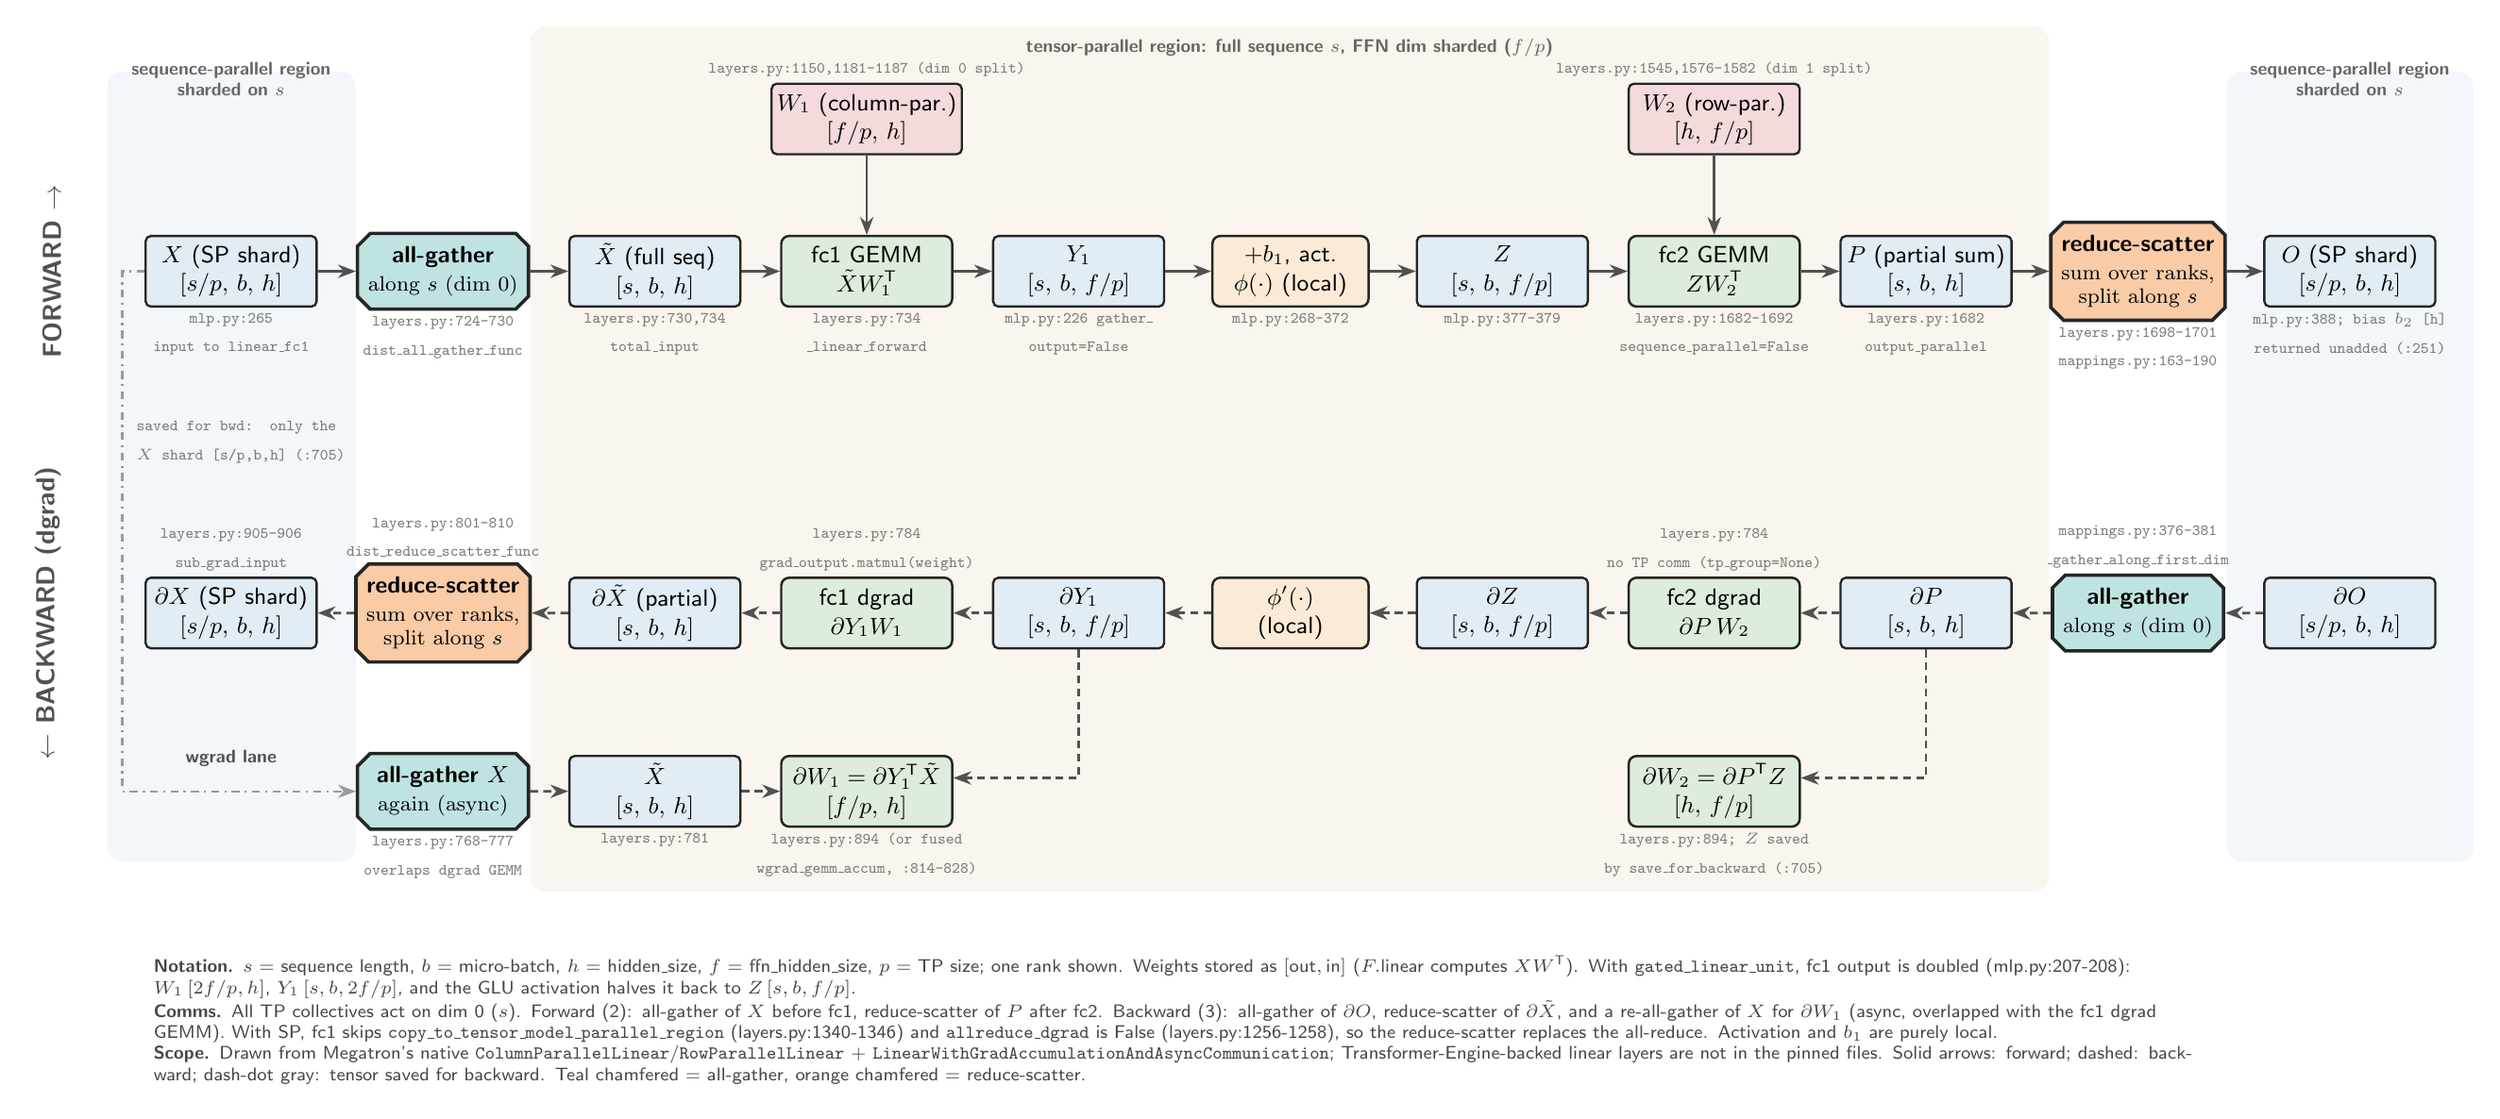
\begin{tikzpicture}[
  >={Stealth[length=2.4mm]},
  font=\sffamily\small,
  tensor/.style={draw=ink,fill=paperblue,rounded corners=2pt,line width=.85pt,minimum width=2.3cm,minimum height=.95cm,align=center,inner sep=2pt},
  weight/.style={draw=ink,fill=paperpink,rounded corners=2pt,line width=.85pt,minimum width=2.3cm,minimum height=.95cm,align=center,inner sep=2pt},
  gemm/.style={draw=ink,fill=papergreen,rounded corners=3pt,line width=.9pt,minimum width=2.3cm,minimum height=.95cm,align=center,inner sep=2pt},
  act/.style={draw=ink,fill=paperpeach,rounded corners=3pt,line width=.9pt,minimum width=2.1cm,minimum height=.95cm,align=center,inner sep=2pt},
  ag/.style={draw=ink,fill=agfill,line width=1.3pt,chamfered rectangle,chamfered rectangle xsep=2pt,minimum width=2.3cm,minimum height=.95cm,align=center,inner sep=2pt,font=\sffamily\small\bfseries},
  rs/.style={draw=ink,fill=rsfill,line width=1.3pt,chamfered rectangle,chamfered rectangle xsep=2pt,minimum width=2.3cm,minimum height=.95cm,align=center,inner sep=2pt,font=\sffamily\small\bfseries},
  flow/.style={draw=ink!80,line width=.95pt,->},
  bflow/.style={draw=ink!80,line width=.95pt,->,densely dashed},
  saved/.style={draw=rulegray,line width=.8pt,->,dash dot},
  cite/.style={text=ink!60,align=center,inner sep=1pt},
  lane/.style={font=\sffamily\bfseries,text=ink!80,anchor=west},
]

% ================= FORWARD (left -> right) =================
\node[tensor] (x)   at (0*\dx,\yF) {$X$ (SP shard)\\\shp{s/p,\,b,\,h}};
\node[ag]     (ag1) at (1*\dx,\yF) {all-gather\\\normalfont\footnotesize along $s$ (dim 0)};
\node[tensor] (xt)  at (2*\dx,\yF) {$\tilde X$ (full seq)\\\shp{s,\,b,\,h}};
\node[gemm]   (fc1) at (3*\dx,\yF) {fc1 GEMM\\$\tilde X W_1^{\mathsf T}$};
\node[tensor] (y1)  at (4*\dx,\yF) {$Y_1$\\\shp{s,\,b,\,f/p}};
\node[act]    (act) at (5*\dx,\yF) {$+b_1$, act.\\$\phi(\cdot)$ (local)};
\node[tensor] (z)   at (6*\dx,\yF) {$Z$\\\shp{s,\,b,\,f/p}};
\node[gemm]   (fc2) at (7*\dx,\yF) {fc2 GEMM\\$Z W_2^{\mathsf T}$};
\node[tensor] (pp)  at (8*\dx,\yF) {$P$ (partial sum)\\\shp{s,\,b,\,h}};
\node[rs]     (rs1) at (9*\dx,\yF) {reduce-scatter\\\normalfont\footnotesize sum over ranks,\\[-2pt]\normalfont\footnotesize split along $s$};
\node[tensor] (o)   at (10*\dx,\yF) {$O$ (SP shard)\\\shp{s/p,\,b,\,h}};

\node[weight] (w1)  at (3*\dx,\yW) {$W_1$ (column-par.)\\\shp{f/p,\,h}};
\node[weight] (w2)  at (7*\dx,\yW) {$W_2$ (row-par.)\\\shp{h,\,f/p}};

% source citations (forward)
\node[cite,below=1pt of x]   {\src{mlp.py:265}\\\src{input to linear\_fc1}};
\node[cite,below=1pt of ag1] {\src{layers.py:724-730}\\\src{dist\_all\_gather\_func}};
\node[cite,below=1pt of xt]  {\src{layers.py:730,734}\\\src{total\_input}};
\node[cite,below=1pt of fc1] {\src{layers.py:734}\\\src{\_linear\_forward}};
\node[cite,below=1pt of y1]  {\src{mlp.py:226 gather\_}\\\src{output=False}};
\node[cite,below=1pt of act] {\src{mlp.py:268-372}};
\node[cite,below=1pt of z]   {\src{mlp.py:377-379}};
\node[cite,below=1pt of fc2] {\src{layers.py:1682-1692}\\\src{sequence\_parallel=False}};
\node[cite,below=1pt of pp]  {\src{layers.py:1682}\\\src{output\_parallel}};
\node[cite,below=1pt of rs1] {\src{layers.py:1698-1701}\\\src{mappings.py:163-190}};
\node[cite,below=1pt of o]   {\src{mlp.py:388; bias $b_2$ [h]}\\\src{returned unadded (:251)}};
\node[cite,above=1pt of w1]  {\src{layers.py:1150,1181-1187 (dim 0 split)}};
\node[cite,above=1pt of w2]  {\src{layers.py:1545,1576-1582 (dim 1 split)}};

\begin{scope}[on background layer]
  \draw[flow] (x) -- (ag1);
  \draw[flow] (ag1) -- (xt);
  \draw[flow] (xt) -- (fc1);
  \draw[flow] (w1) -- (fc1);
  \draw[flow] (fc1) -- (y1);
  \draw[flow] (y1) -- (act);
  \draw[flow] (act) -- (z);
  \draw[flow] (z) -- (fc2);
  \draw[flow] (w2) -- (fc2);
  \draw[flow] (fc2) -- (pp);
  \draw[flow] (pp) -- (rs1);
  \draw[flow] (rs1) -- (o);
\end{scope}

% ================= BACKWARD dgrad (right -> left) =================
\node[tensor] (go)  at (10*\dx,\yB) {$\partial O$\\\shp{s/p,\,b,\,h}};
\node[ag]     (ag2) at (9*\dx,\yB)  {all-gather\\\normalfont\footnotesize along $s$ (dim 0)};
\node[tensor] (gp)  at (8*\dx,\yB)  {$\partial P$\\\shp{s,\,b,\,h}};
\node[gemm]   (d2)  at (7*\dx,\yB)  {fc2 dgrad\\$\partial P\, W_2$};
\node[tensor] (gz)  at (6*\dx,\yB)  {$\partial Z$\\\shp{s,\,b,\,f/p}};
\node[act]    (dact) at (5*\dx,\yB) {$\phi'(\cdot)$\\(local)};
\node[tensor] (gy1) at (4*\dx,\yB)  {$\partial Y_1$\\\shp{s,\,b,\,f/p}};
\node[gemm]   (d1)  at (3*\dx,\yB)  {fc1 dgrad\\$\partial Y_1 W_1$};
\node[tensor] (gxt) at (2*\dx,\yB)  {$\partial\tilde X$ (partial)\\\shp{s,\,b,\,h}};
\node[rs]     (rs2) at (1*\dx,\yB)  {reduce-scatter\\\normalfont\footnotesize sum over ranks,\\[-2pt]\normalfont\footnotesize split along $s$};
\node[tensor] (gx)  at (0*\dx,\yB)  {$\partial X$ (SP shard)\\\shp{s/p,\,b,\,h}};

\node[cite,above=1pt of ag2] {\src{mappings.py:376-381}\\\src{\_gather\_along\_first\_dim}};
\node[cite,above=1pt of d2]  {\src{layers.py:784}\\\src{no TP comm (tp\_group=None)}};
\node[cite,above=1pt of d1]  {\src{layers.py:784}\\\src{grad\_output.matmul(weight)}};
\node[cite,above=1pt of rs2] {\src{layers.py:801-810}\\\src{dist\_reduce\_scatter\_func}};
\node[cite,above=1pt of gx]  {\src{layers.py:905-906}\\\src{sub\_grad\_input}};

\begin{scope}[on background layer]
  \draw[bflow] (go) -- (ag2);
  \draw[bflow] (ag2) -- (gp);
  \draw[bflow] (gp) -- (d2);
  \draw[bflow] (d2) -- (gz);
  \draw[bflow] (gz) -- (dact);
  \draw[bflow] (dact) -- (gy1);
  \draw[bflow] (gy1) -- (d1);
  \draw[bflow] (d1) -- (gxt);
  \draw[bflow] (gxt) -- (rs2);
  \draw[bflow] (rs2) -- (gx);
\end{scope}

% ================= BACKWARD wgrad =================
\node[ag]     (ag3) at (1*\dx,\yG) {all-gather $X$\\\normalfont\footnotesize again (async)};
\node[tensor] (xt2) at (2*\dx,\yG) {$\tilde X$\\\shp{s,\,b,\,h}};
\node[gemm]   (dw1) at (3*\dx,\yG) {$\partial W_1=\partial Y_1^{\mathsf T}\tilde X$\\\shp{f/p,\,h}};
\node[gemm]   (dw2) at (7*\dx,\yG) {$\partial W_2=\partial P^{\mathsf T} Z$\\\shp{h,\,f/p}};

\node[cite,below=1pt of ag3] {\src{layers.py:768-777}\\\src{overlaps dgrad GEMM}};
\node[cite,below=1pt of dw1] {\src{layers.py:894 (or fused}\\\src{wgrad\_gemm\_accum, :814-828)}};
\node[cite,below=1pt of dw2] {\src{layers.py:894; $Z$ saved}\\\src{by save\_for\_backward (:705)}};
\node[cite,below=1pt of xt2] {\src{layers.py:781}};

\begin{scope}[on background layer]
  \draw[bflow] (ag3) -- (xt2);
  \draw[bflow] (xt2) -- (dw1);
  \draw[bflow] (gy1.south) |- ($(dw1.east)+(0,.18)$);
  \draw[bflow] (gp.south) |- ($(dw2.east)+(0,.18)$);
  % only the s/p shard of X is saved for backward (layers.py:705)
  \draw[saved] (x.west) -- ++(-.3,0) |- (ag3.west);
\end{scope}
\node[cite,anchor=west,align=left] at ($(x.west)+(-.15,-2.3)$) {\src{saved for bwd: only the}\\\src{$X$ shard [s/p,b,h] (:705)}};

% ================= regions & lanes =================
\begin{pgfonlayer}{regions}
  \fill[spregion,rounded corners=6pt] ($(x.north west)+(-.5,2.2)$) rectangle ($(ag1.west)+(-.0,-7.95)$);
  \fill[spregion,rounded corners=6pt] ($(o.north east)+(.5,2.2)$) rectangle ($(rs1.east)+(.0,-7.95)$);
  \fill[tpregion,rounded corners=6pt] ($(ag1.east)+(0,3.3)$) rectangle ($(rs1.west)+(0,-8.35)$);
\end{pgfonlayer}
\node[font=\sffamily\scriptsize\bfseries,text=ink!70,align=center,anchor=south] at ($(x.north)+(0,1.75)$) {sequence-parallel region\\sharded on $s$};
\node[font=\sffamily\scriptsize\bfseries,text=ink!70,align=center,anchor=south] at ($(o.north)+(0,1.75)$) {sequence-parallel region\\sharded on $s$};
\node[font=\sffamily\scriptsize\bfseries,text=ink!70,anchor=north] at ($(ag1.east)!.5!(rs1.west)+(0,3.25)$) {tensor-parallel region: full sequence $s$, FFN dim sharded ($f/p$)};

\node[lane,rotate=90,anchor=south] at ($(x.west)+(-1.0,0)$) {FORWARD $\rightarrow$};
\node[lane,rotate=90,anchor=south] at ($(gx.west)+(-1.0,0)$) {$\leftarrow$ BACKWARD (dgrad)};
\node[font=\sffamily\scriptsize\bfseries,text=ink!80] at (0,\yG+.45) {wgrad lane};

% ================= legend / notes =================
\node[anchor=north west,align=left,font=\sffamily\scriptsize,text=ink!85,text width=27.5cm]
  at ($(gx.south west)+(0,-4.0)$) {%
  \textbf{Notation.} $s$ = sequence length, $b$ = micro-batch, $h$ = hidden\_size, $f$ = ffn\_hidden\_size, $p$ = TP size; one rank shown. Weights stored as $[\text{out},\text{in}]$ ($F.\text{linear}$ computes $XW^{\mathsf T}$).
  With \texttt{gated\_linear\_unit}, fc1 output is doubled (mlp.py:207-208): $W_1\,[2f/p,h]$, $Y_1\,[s,b,2f/p]$, and the GLU activation halves it back to $Z\,[s,b,f/p]$.\\
  \textbf{Comms.} All TP collectives act on dim 0 ($s$). Forward (2): all-gather of $X$ before fc1, reduce-scatter of $P$ after fc2. Backward (3): all-gather of $\partial O$, reduce-scatter of $\partial\tilde X$, and a re-all-gather of $X$ for $\partial W_1$ (async, overlapped with the fc1 dgrad GEMM).
  With SP, fc1 skips \texttt{copy\_to\_tensor\_model\_parallel\_region} (layers.py:1340-1346) and \texttt{allreduce\_dgrad} is False (layers.py:1256-1258), so the reduce-scatter replaces the all-reduce. Activation and $b_1$ are purely local.\\
  \textbf{Scope.} Drawn from Megatron's native \texttt{ColumnParallelLinear}/\texttt{RowParallelLinear} + \texttt{LinearWithGradAccumulationAndAsyncCommunication}; Transformer-Engine-backed linear layers are not in the pinned files.
  Solid arrows: forward; dashed: backward; dash-dot gray: tensor saved for backward. Teal chamfered = all-gather, orange chamfered = reduce-scatter.};

\end{tikzpicture}
\end{document}
